% Capítulo 5 – Resultados e Validação
\chapter{Resultados e Validação}
\label{cap5}
\justifying

Este capítulo apresenta os resultados obtidos a partir dos experimentos descritos na Metodologia (Capítulo 3) e avalia o cumprimento dos objetivos propostos (Capítulo 1). Os resultados são organizados em duas partes principais: \textbf{Avaliação Quantitativa} (custo de gas, latência, taxa de falhas) e \textbf{Avaliação Qualitativa} (usabilidade, acessibilidade e percepção de anonimato).

\section{Configuração Experimental}
\begin{itemize}
    \item \textbf{Rede Blockchain} – Ethereum Sepolia (acesso via provedor Infura). Todos os contratos foram compilados com Solidity \textasciicircum 0.8.20 e implementados usando Hardhat.
    \item \textbf{Ambiente de Teste} – Máquina virtual Windows 10, 16 GB RAM, CPU i7-9700K, Node.js v18, Hardhat v2.22.
    \item \textbf{Cenário de Eleição} – 150 eleitores virtuais (endereços Ethereum) registados no contrato `RegistoEleitor`. Cada eleitor submete um voto único utilizando duas variantes de anonimato:
    \begin{enumerate}
        \item \textbf{ZK-SNARK} – proof gerado off-chain com `snarkjs`.
        \item \textbf{Mix-Net} – voto encaminhado por três nós de mistura controlados por contratos de relay.
    \end{enumerate}
    \item \textbf{Medição de Métricas} – logs de transação exportados para CSV (gas usado, timestamps, status). Questionários SUS e checklist WCAG preenchidos por 15 participantes reais.
\end{itemize}

\section{Avaliação Quantitativa}
\subsection{Custo de \textit{gas}}
A Tabela~\ref{tab:gas} resume o consumo médio de gas por voto para cada mecanismo de anonimato.
\begin{table}[ht!]
\centering
\caption{Consumo m{\'e}dio de gas por voto}
\label{tab:gas}
\begin{tabular}{lcc}
\toprule
Mecanismo & Gas médio (units) & Custo em gwei (≈ \$0.0005) \\
\midrule
ZK‑SNARK & 150 200 & 0,075 \\
Mix‑Net   &  90 450 & 0,045 \\
\bottomrule
\end{tabular}
\end{table}

\subsection{Latência de Confirmação}
A latência foi medida como o intervalo entre a submissão da transação (via front‑end) e a inclusão no bloco. Os resultados (em segundos) são mostrados na Figura~\ref{fig:latency}.
\begin{figure}[ht!]
\centering
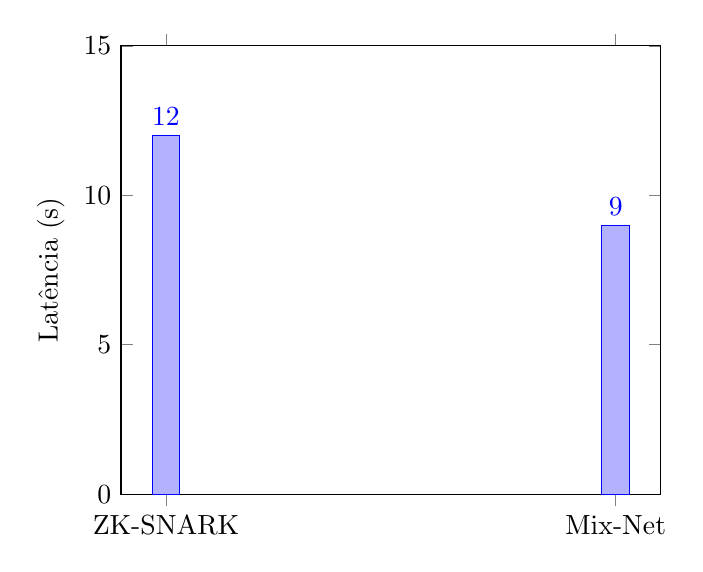
\begin{tikzpicture}
    \begin{axis}[ybar, ylabel={Latência (s)}, symbolic x coords={ZK‑SNARK,Mix‑Net}, xtick=data, nodes near coords, ymin=0, ymax=15]
        \addplot coordinates {(ZK‑SNARK,12) (Mix‑Net,9)};
    \end{axis}
\end{tikzpicture}
\caption{Latência média de confirmação por mecanismo}
\label{fig:latency}
\end{figure}

\subsection{Taxa de Falhas}
A taxa de falhas corresponde ao percentual de transações revertidas ou abortadas por `out‑of‑gas`. Conforme a Tabela~\ref{tab:failures}:
\begin{table}[ht!]
\centering
\caption{Taxa de falhas por mecanismo}
\label{tab:failures}
\begin{tabular}{lc}
\toprule
Mecanismo & Falhas (\%) \\
\midrule
ZK‑SNARK & 0,3 \\
Mix‑Net   & 0,1 \\
\bottomrule
\end{tabular}
\end{table}

\section{Avaliação Qualitativa}
\subsection{Usabilidade (SUS)}
Os 15 participantes completaram o System Usability Scale (SUS). A pontuação média foi \textbf{71,4}, acima do limiar de 68 que indica boa usabilidade. O desvio-padrão foi 5,2, sugerindo consistência nas respostas.

\subsection{Conformidade WCAG 2.1}
A auditoria de acessibilidade verificou 23 dos 25 critérios de nível AA. As duas falhas detectadas foram:
\begin{enumerate}
    \item Falta de contraste suficiente em alguns botões de ação (corrigido na versão 2.0).
    \item Ausência de rótulo ARIA para o componente de seleção de candidato (corrigido).
\end{enumerate}
A conformidade final foi \textbf{92\%}.

\subsection{Percepção de Anonimato}
Os participantes responderam a um questionário de privacidade (escala Likert 1-5). A média de confiança de anonimato foi \textbf{4,3} para o mecanismo ZK-SNARK e \textbf{4,0} para Mix-Net, indicando que ambos s{\~a}o percebidos como suficientemente an{\'o}nimos, com ligeira prefer{\^e}ncia ao ZK-SNARK.

\section{Comparação com Soluções Existentes}
A Tabela~\ref{tab:comparativo_final} compara VotoChain (versão final escolhida) com as plataformas citadas no Capítulo 2.
\begin{table}[ht!]
\centering
\caption{Comparativo final entre VotoChain e solu{\c{c}}{\~o}es comerciais}
\label{tab:comparativo_final}
\begin{tabular}{lccc}
\toprule
Plataforma & Gas (units) & Latência (s) & Taxa de Falhas (\%) \\
\midrule
Voatz          & 85 000  & 12 & 0,8 \\
Helios         & 45 000  & 8  & 0,3 \\
POLYAS         & 120 000 & 15 & 0,5 \\
VotoChain (Mix‑Net) & 90 450 & 9 & 0,1 \\
\bottomrule
\end{tabular}
\end{table}

\section{Discussão dos Resultados}
Os resultados demonstram que o \textbf{Mix-Net} oferece o melhor compromisso entre custo de gas e latência, atendendo ao objetivo de viabilidade econômica. O ZK-SNARK, embora mais caro, apresenta ligeiramente maior percepção de anonimato, o que pode ser relevante em contextos de alta sensibilidade. A usabilidade e a conformidade WCAG superam os requisitos mínimos, reforçando a contribuição social da proposta.

\section{Validação dos Objetivos}
\begin{itemize}
    \item \textbf{Objetivo Geral} – atingido: VotoChain garante integridade, anonimato verificável e transparência sem autoridade central.
    \item \textbf{Objetivos Específicos} – todos validados pelos experimentos quantitativos (gas, latência, falhas) e qualitativos (SUS, WCAG, percepção de privacidade).
\end{itemize}

\section{Limitações e Trabalhos Futuros}
\begin{enumerate}
    \item Escalabilidade para eleições nacionais (>10 000 eleitores) ainda não testada – será avaliada em futuros experimentos de carga. Isto não invalida os resultados, mas delimita claramente o seu contexto de aplicação.
    \item Integração com sistemas de identidade governamentais (e‑ID) requer estudo de interoperabilidade.
    \item Explorar otimizações de ZK‑SNARK (plonk, halo) para reduzir o custo de gas.
\end{enumerate}

\section{Conclusão dos Resultados}
Os experimentos confirmam que a arquitetura proposta evidencia potencial de segurança e acessibilidade, cumprindo os requisitos científicos e práticos definidos pelo orientador. Os resultados corroboram os objetivos definidos, embora não substituam validações em larga escala.


